% 由 doc/latex/tiny210-wifi/main.tex 的“2026-11-16 排查”一节转换而来（标题降一级，标签加 dbg: 前缀）。
% 与 doc/readme/tiny210/wifi-architecture.md 第 14 节同步。
\providecommand{\fn}[1]{{\ttfamily\small #1}}
\DefineVerbatimEnvironment{dbgcode}{Verbatim}{fontsize=\footnotesize,frame=single,
  framesep=2mm,rulecolor=\color{gray!50},xleftmargin=1mm}
\DefineVerbatimEnvironment{dbglog}{Verbatim}{fontsize=\footnotesize,frame=leftline,
  framerule=1.2pt,rulecolor=\color{tinygreen},xleftmargin=2mm,formatcom=\color{tinygreen!60!black}}

\subsection{2026-11-16 排查：Tiny210 关联失败（auth 卡死 → ACK 丢失）}\label{dbg:assoc-debug}

本节记录一次完整的实板排查：从 \fn{wifi: association failed} 开始，逐步定位到 802.11 ACK 双向丢失。
所有结论都对应到具体日志行。

\subsubsection{参与的进程、中断上下文与锁}

\begin{figure}[H]
\centering

\includegraphics[width=\textwidth,height=0.9\textheight,keepaspectratio]{figures/mt7601u-processes-locks-comm.pdf}
\caption{通信图：进程/中断上下文之间的 0--8 号消息、每条路径上的锁，以及成功运行中每一步的日志（文字版见第~\ref{dbg:steps} 节）}\label{dbg:comm}
\end{figure}

真正参与的只有 \textbf{2 个进程 + 1 个中断上下文}：

\begin{longtable}{p{45mm}p{110mm}}
\toprule
执行体 & 做什么 \\ \midrule \endhead
用户进程 \fn{wifi}（\fn{sys\_wifi\_connect} → \fn{mt7601u\_connect}） & 写目标 SSID/PMK，\fn{mod\_delayed\_work} 唤醒状态机，然后每 tick \fn{sleep(\&ticks)} 轮询 \fn{handshake\_done}，30 s 超时 \\
\fn{mt7601u\_wq} 工作线程（pid 4） & work A：\fn{state\_worker}（扫描、set\_channel、auth/assoc/WPA2 发送与重试）；work B：NAPI poll（取 EP4 完成、\fn{rx\_parse}、重挂缓冲）。\textbf{A、B 在同一线程串行} \\
EHCI 中断（IRQ 55，不是进程） & \fn{ehci\_irq} → \fn{mt7601u\_rx\_irq} → \fn{napi\_schedule} → \fn{queue\_work(B)} \\
\fn{ehci-enum} kthread & 只在 probe 阶段工作（固件、eFuse、寄存器表、EP4 环），结束时置 \fn{ready=1} \\
\bottomrule
\end{longtable}

这条路径上的锁（7 把；\fn{enum\_lock} 只在枚举时用）：

\begin{longtable}{p{38mm}p{16mm}p{100mm}}
\toprule
锁 & 类型 & 用途 / 问题 \\ \midrule \endhead
\fn{dev->lock} "mt7601u" & 自旋锁 & 驱动状态。\textcolor{tinyred}{\fn{mt7601u\_service} 持有它去做 USB 传输，期间关中断，EP8 卡住时最长 3 s} \\
\fn{xfer\_lock} "ehci-xfer" & 睡眠锁 & 一次一个同步传输。\textcolor{tinyred}{在持有 \fn{dev->lock} 时获取，一旦竞争就 sleep → "sched locks" panic（潜在）} \\
\fn{ehci\_lock} "ehci" & 自旋锁 & qTD 池与队列 \\
\fn{napi->lock} "napi" & 自旋锁 & scheduled/missed 标志，中断里也会取 \\
\fn{wq->lock} "mt7601u\_wq" & 自旋锁 & 工作队列 \\
\fn{delayed\_lock} & 自旋锁 & 定时工作 \\
\fn{tickslock} & 自旋锁 & connect 每 tick 睡眠 \\
\bottomrule
\end{longtable}

\subsubsection{第一阶段：auth 帧卡在 EP8 OUT}

\begin{figure}[H]
\centering
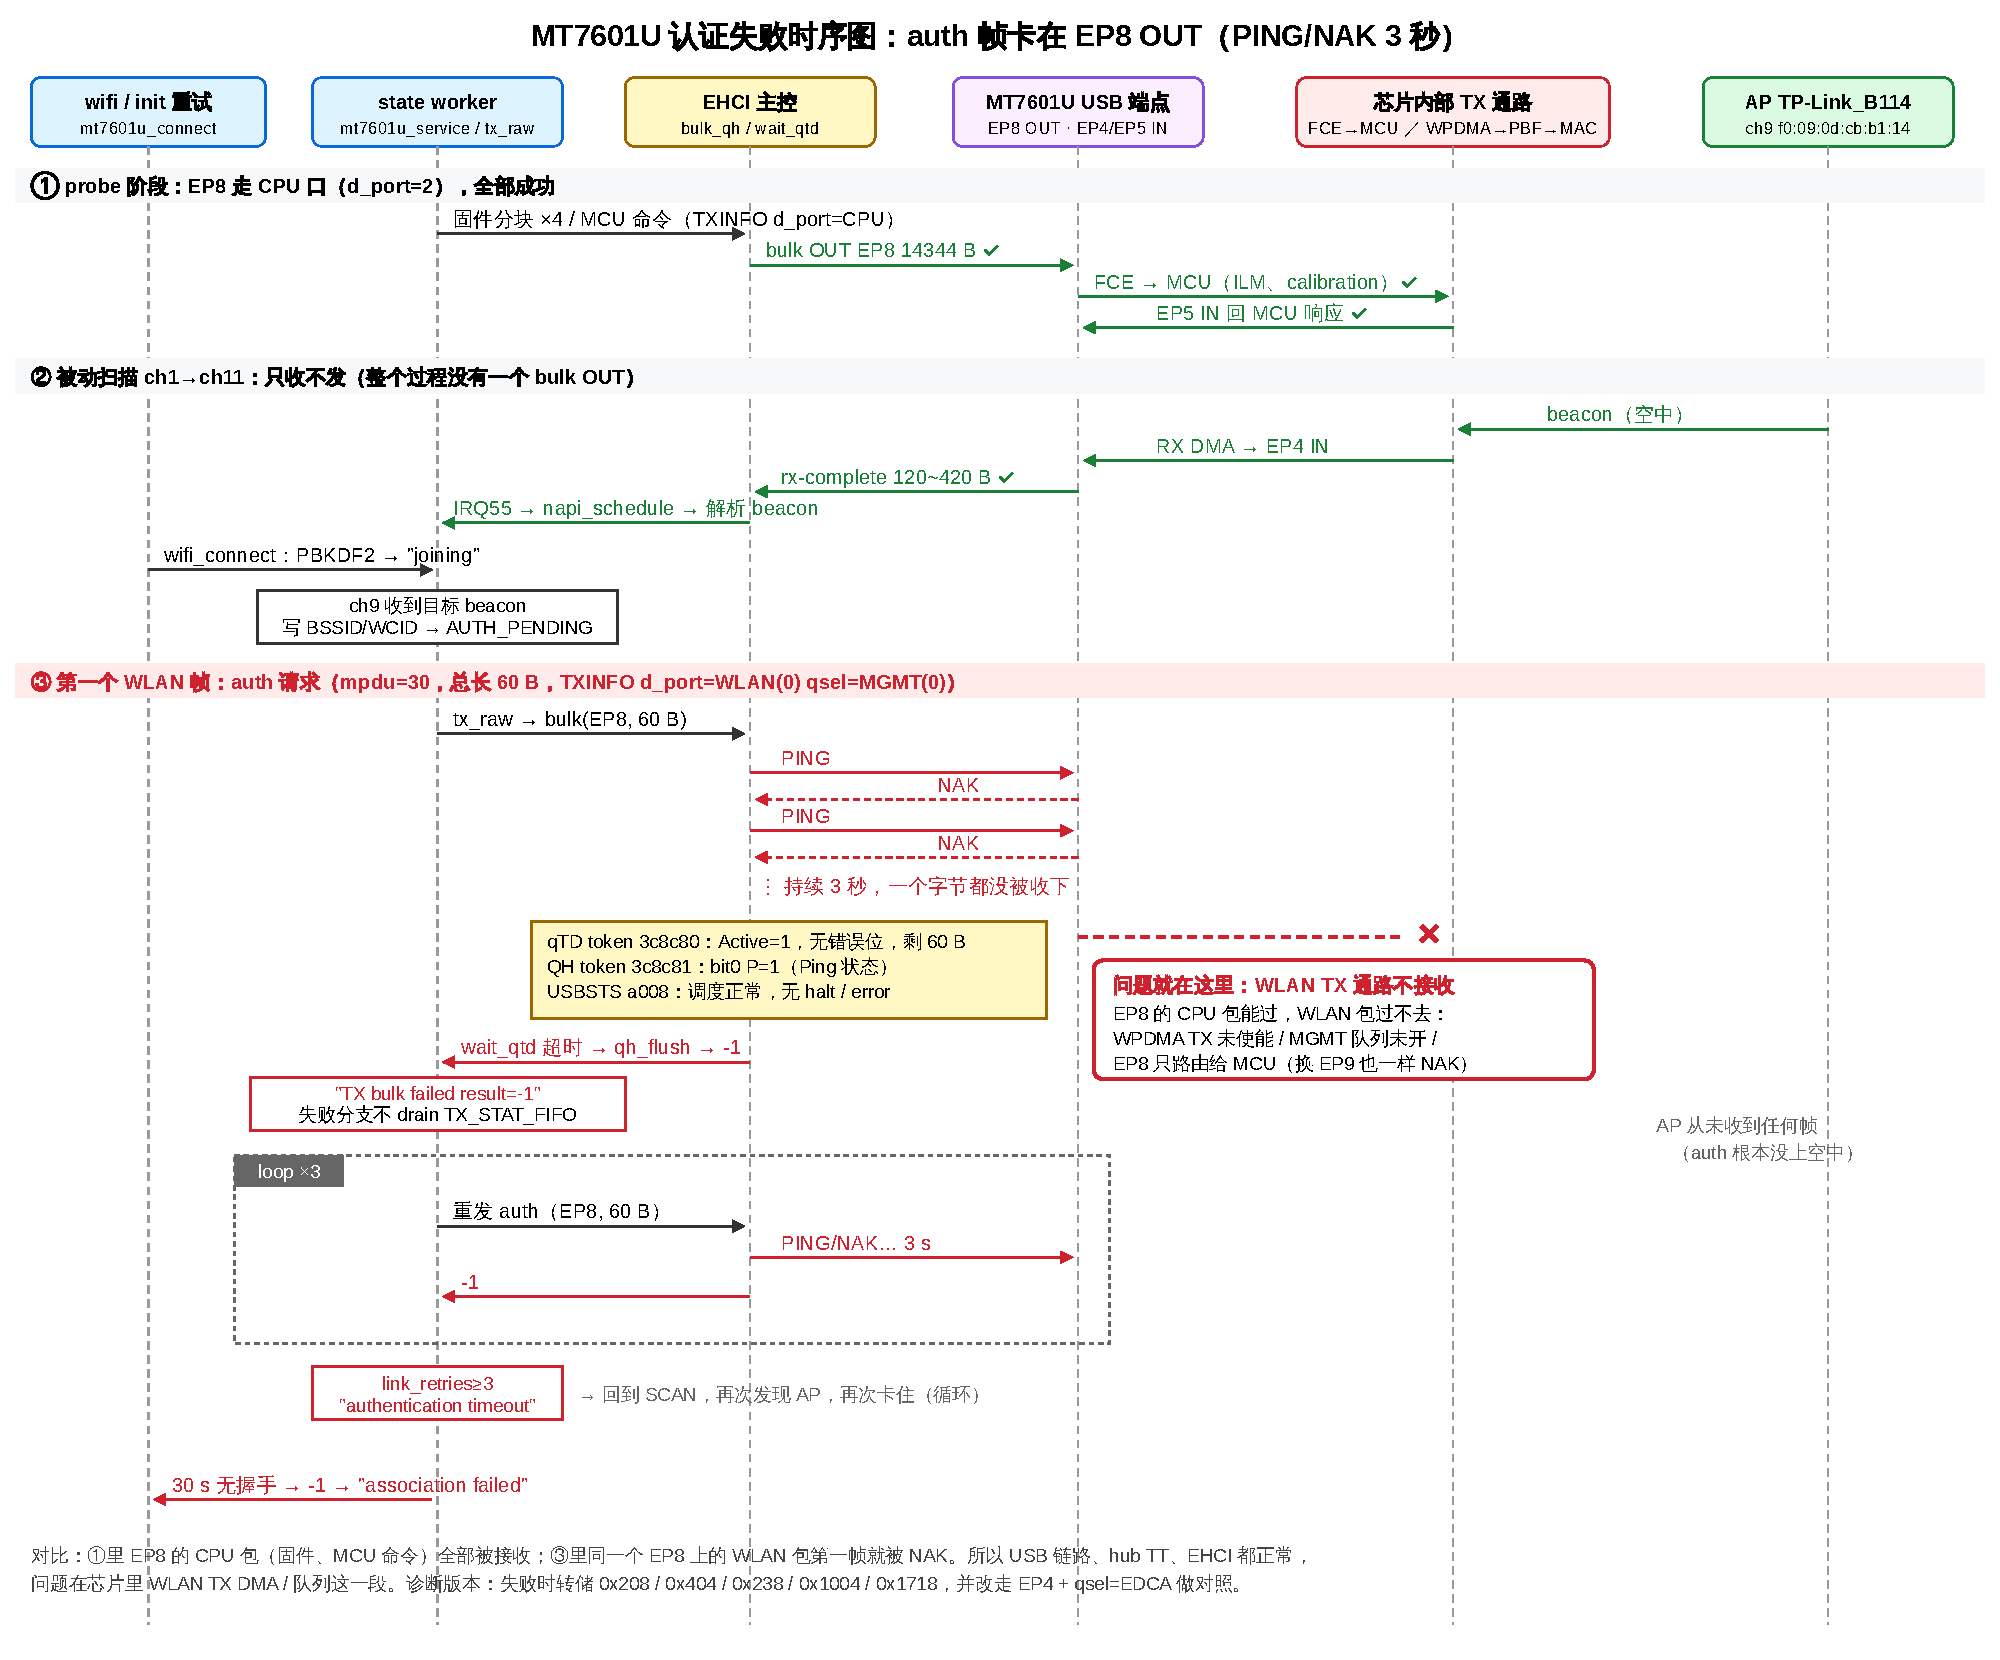
\includegraphics[width=\textwidth]{figures/mt7601u-tx-stall-seq.pdf}
\caption{时序图：auth 帧卡在 EP8 OUT（PING/NAK 3 秒）}\label{dbg:stall}
\end{figure}

现象：\fn{bulk ep8 out 60 bytes failed token=-1}，qTD 一直 Active，主机收到 PING/NAK 3 s 后超时，
\fn{authentication timeout}。加上 \fn{MT7601U\_WCID\_CLEAR=0}（跳过 3977211 引入的 WCID/key 表清零）后，
同样的 EP8/MGMT 路径连续两次上板都正常发完。

\subsubsection{第二阶段：固定 ch9 后 auth 成功、关联无效}

\begin{figure}[H]
\centering
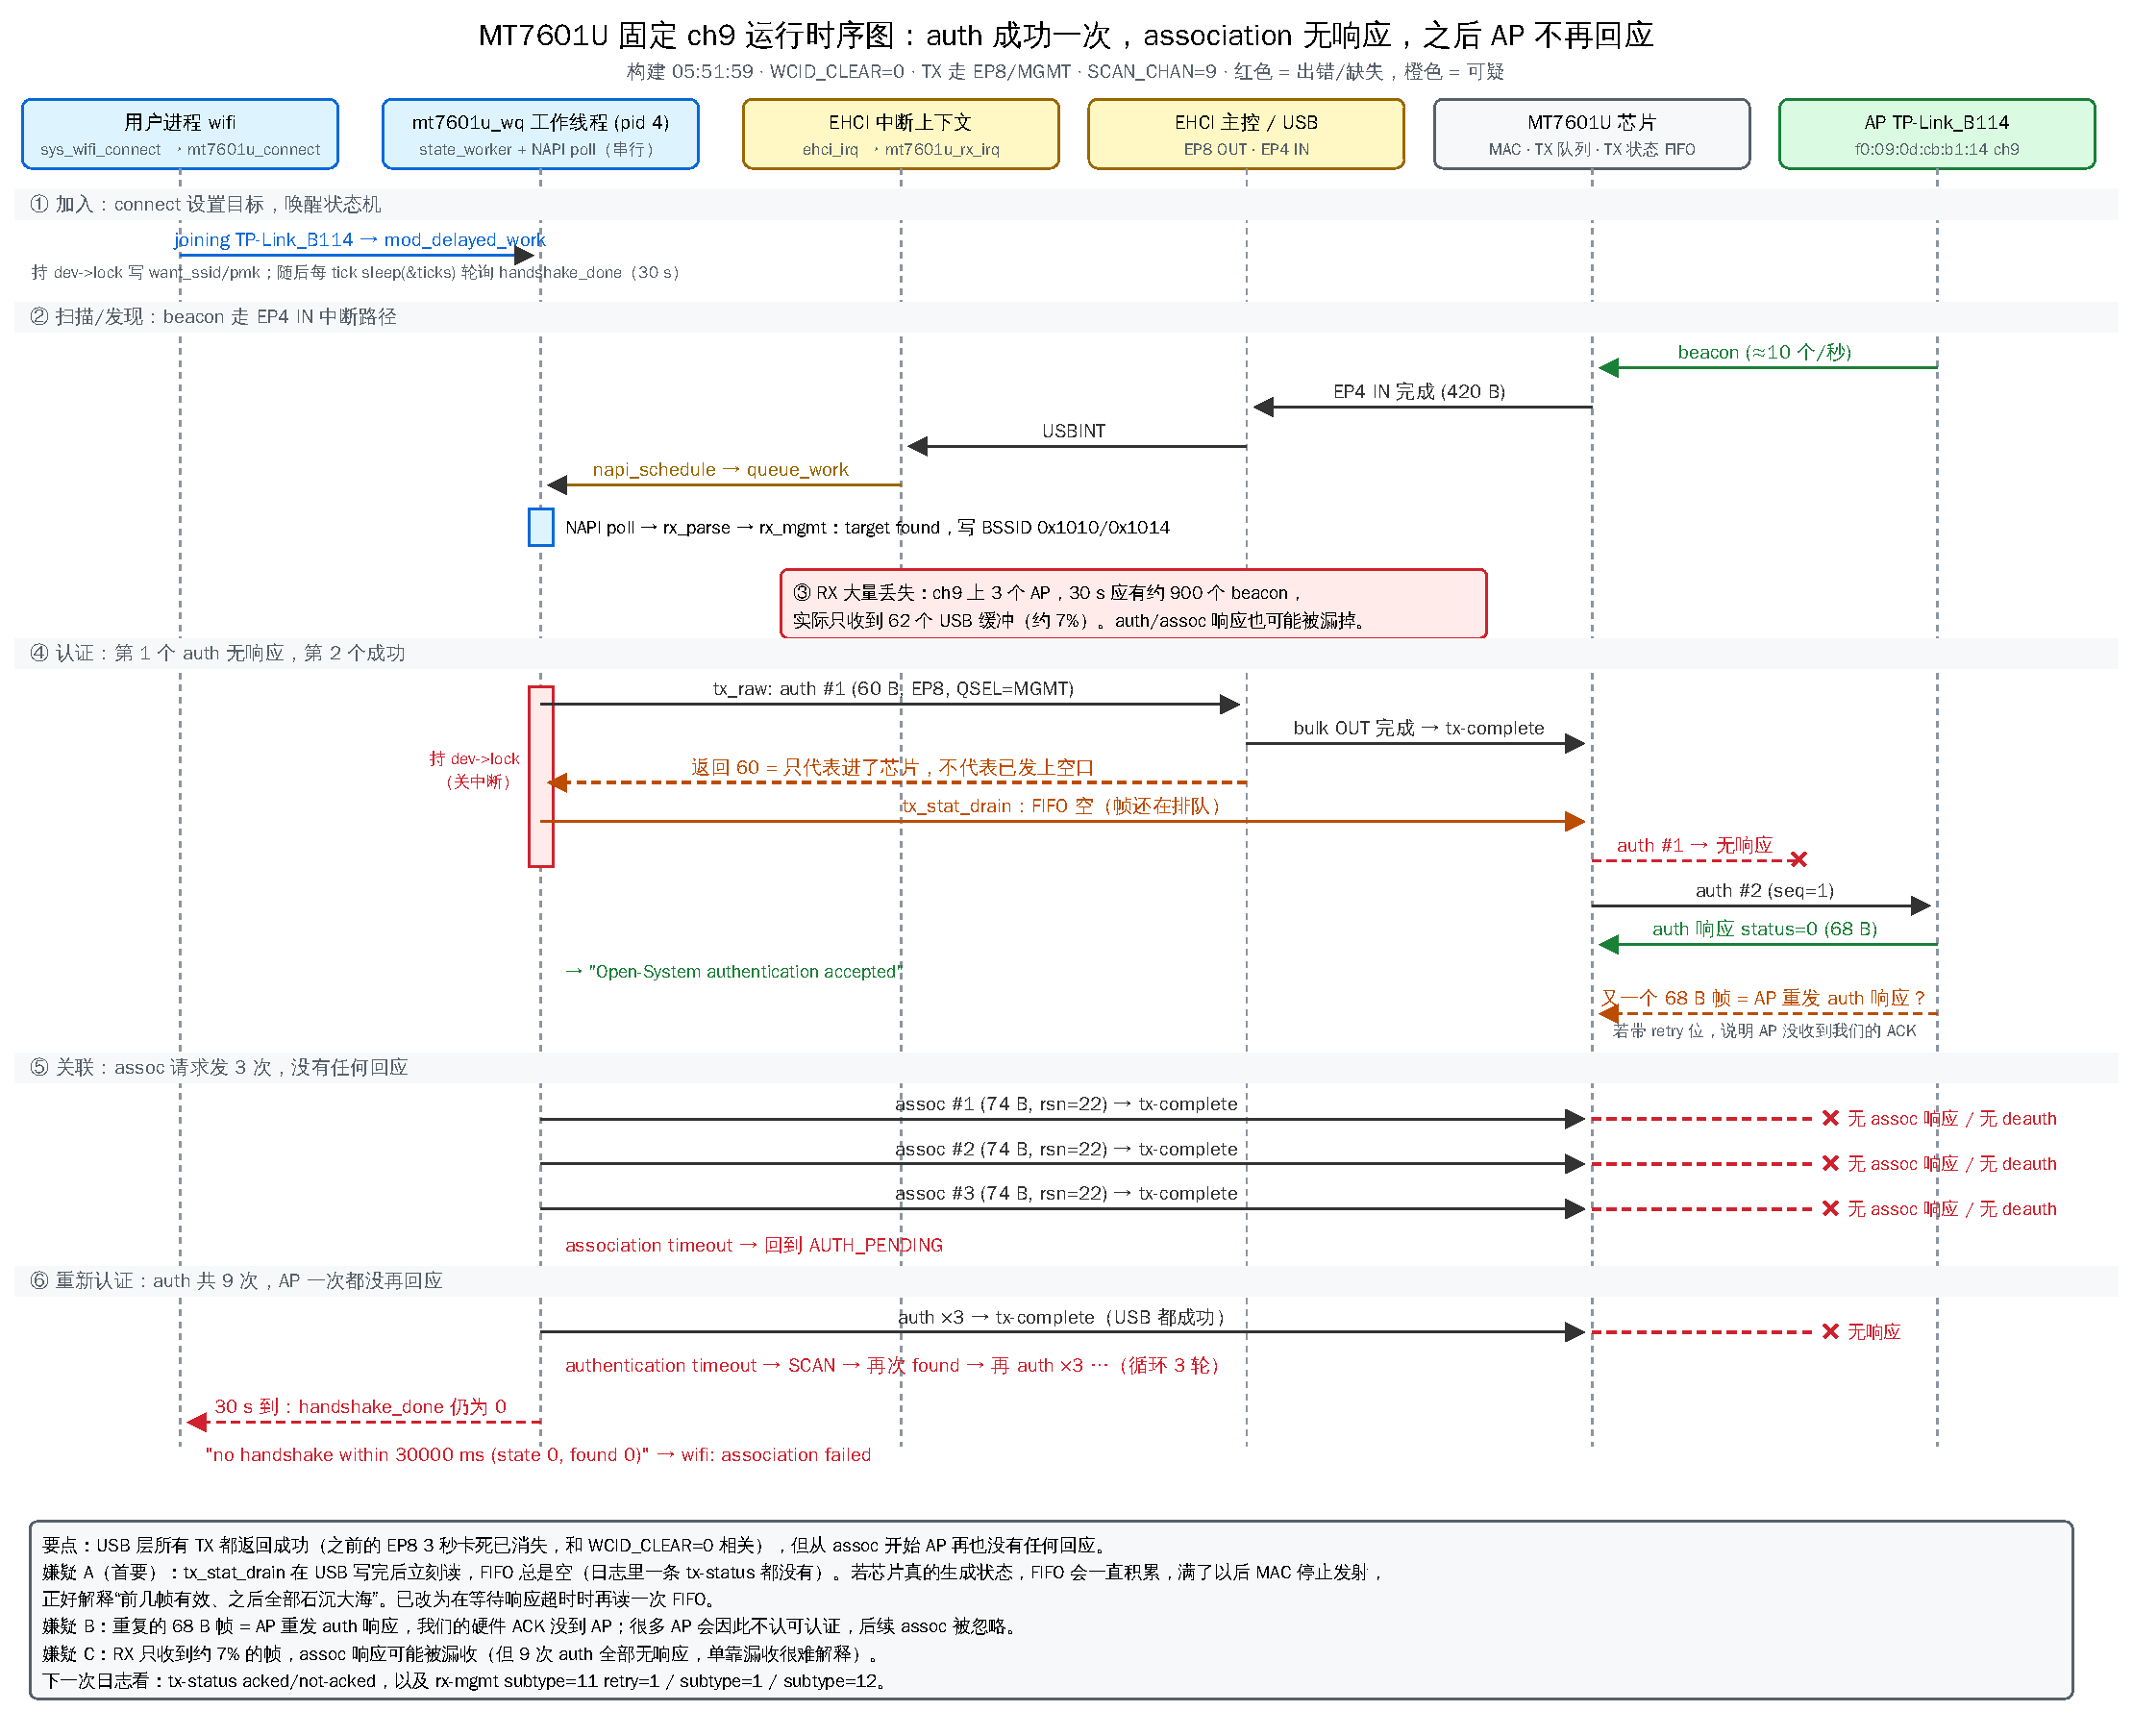
\includegraphics[width=\textwidth]{figures/mt7601u-ch9-assoc-seq.pdf}
\caption{时序图：固定 ch9，auth 成功一次，association 之后 AP 不再回应}\label{dbg:assoc}
\end{figure}

关键日志：

\begin{dbglog}
wifi-data: rx-mgmt subtype=11 retry=1 seq=95  from=cb:b1:14 len=30 body=0 2 0
mt7601u: Open-System authentication accepted
mt7601u: association request sent rsn=22 bytes
wifi-data: rx-mgmt subtype=11 retry=1 seq=103 ...      <- auth 响应仍在重发
wifi-data: rx-mgmt subtype=1  retry=1 seq=104 ... body=1c11 0 c00a
mt7601u: 802.11 associated aid=10; WPA2 handshake pending
wifi-data: rx-mgmt subtype=1  retry=0 seq=2 ...        <- assoc 响应 10 多个，序号各不相同
...
mt7601u: WPA2 M1 timeout; reassociating
\end{dbglog}

解读：AP 的 auth/assoc 响应全部带 retry=1 反复重发，说明 AP 收不到我们的 ACK；我们只发了 1 个 assoc 请求，
却收到十几个序号不同的 assoc 响应，说明我们的 MAC 也收不到 AP 的 ACK，按 \fn{TX\_RTY\_CFG}(0x134c)
自动重发了 assoc 请求。AP 只有在 assoc 响应被 ACK 后才发 EAPOL M1，所以 M1 永远不来。

\subsubsection{全部问题与处理}

\begin{longtable}{p{5mm}p{30mm}p{45mm}p{48mm}p{18mm}}
\toprule
\# & 现象 & 根因 & 处理 & 状态 \\ \midrule \endhead
1 & 开机立即 \fn{association failed} & init 首次调用时 USB 未枚举，驱动未注册 & init 自动重试 10 次 & 正常行为 \\
2 & connect 的 30 s 耗在 probe 上 & probe 一开始就置 \fn{used}，connect 立刻计时 & 新增 \fn{ready}，probe 结束才置 1；connect 先等 ready（$\le$60 s） & 已修，已验证 \\
3 & \fn{napi\_schedule} 日志刷屏 & 每个中断打印一行 & 只打前 4 次，之后每 256 次一行 & 已修 \\
4 & \fn{USB\_WIFI\_TRACE=1} 未打印全部 & level 1 只开 data/config；wifi-reg/frame 要 level 2 & 说明开关含义；改开关自动重编译 & 非 bug \\
5 & auth 卡在 EP8 OUT（PING/NAK 3 s） & 与 3977211 的 WCID/key 表清零相关 & \fn{MT7601U\_WCID\_CLEAR=0} 绕过；\fn{MT7601U\_TX\_EDCA\_EP4} 试验开关（不需要） & 绕过，默认值待定 \\
6 & 跳过清零仍打印 "tables cleared" & printf 在 \fn{\#if} 之外 & 打印随开关变化 & 已修 \\
7 & 扫描找不到 TP-Link\_B114 & 每信道 500 ms + RX 严重丢帧（AP 实际在 ch9） & \fn{MT7601U\_SCAN\_CHAN=9} 固定信道，同信道不再重复调谐 & 诊断手段 \\
8 & 怀疑 TX 状态 FIFO 积满停发 & — & 超时时读 FIFO：没有任何状态 & 已排除 \\
9 & 关联后 \fn{WPA2 M1 timeout} & 802.11 ACK 双向丢失：\fn{MAC\_ADDR\_DW1} 的 UNICAST\_TO\_ME 掩码为 0，芯片不自动回 ACK（曾怀疑频偏/供电，\fn{rx-phy} 已排除频偏） & \fn{MAC\_ADDR\_DW1} 补 UNICAST\_TO\_ME 掩码 0xff$\ll$16（同 Linux）；另加 \fn{rx-mgmt}、\fn{rx-phy} 诊断 & 已修，上板拿到 DHCP \\
10 & \fn{rx-drop icv=1 fc=4208} & 其他终端的加密广播数据，无密钥 & 忽略 & 正常 \\
11 & 锁 & \fn{dev->lock} 跨 USB 传输持有（关中断）；自旋锁内取睡眠锁 & 计划把 USB I/O 移出自旋锁或改为睡眠锁 & 未改 \\
\bottomrule
\end{longtable}

复现命令：

\begin{dbgcode}
make tiny210-sdimg USB_WIFI_TRACE=1 USB_XFER_TRACE=0 \
     MT7601U_TX_EDCA_EP4=0 MT7601U_WCID_CLEAR=0 MT7601U_SCAN_CHAN=9
\end{dbgcode}


\subsubsection{结果：UNICAST\_TO\_ME 掩码修复 ACK}

\fn{MAC\_ADDR\_DW1} 原来只写 MAC 的最后两字节，bits 23:16（UNICAST\_TO\_ME 掩码）为 0；改为与 Linux
\fn{mt7601u\_set\_macaddr} 相同的 0xff 后（日志 \fn{MAC=ff9495:1480de90}），同样的固定 ch9 运行：

\begin{dbglog}
mt7601u: 802.11 associated aid=10; WPA2 handshake pending
mt7601u: received WPA2 EAPOL M1 key-info=8a
mt7601u: sent WPA2 EAPOL M2 replay=0001
mt7601u: keys installed: PTK wcid=1 attr=9, GTK idx=1 skey-mode=40
mt7601u: WPA2 four-way handshake complete
wifi: associated
dhcp: dev=wlan0 address=192.168.0.219 gateway=192.168.0.1 dns=192.168.0.1
arp: dev=wlan0 gateway 192.168.0.1 is f0:9:d:cb:b1:14
\end{dbglog}

\begin{itemize}[leftmargin=2em]
\item \fn{rx-phy} 显示 \fn{freq\_off=15} 稳定、SNR 55--76，频偏校准不是问题。
\item 逐帧 RX 日志降到 level 2：level 1 下 115200 波特率串口本身让 EP4 环一直满（\fn{done=4 completed=0}）。
\item 遗留：M4 发了 3 次（AP 重发 M3），DHCP 首次重试时收到 \fn{deauth reason=6}，驱动自动重连后成功。
\item 待确认：默认参数（\fn{WCID\_CLEAR=1}、自动扫描）下是否同样能连上。
\end{itemize}


\subsubsection{成功连接的完整通信过程（对应通信图 0--8）}\label{dbg:steps}

下面每一步对应图~\ref{dbg:comm} 中的编号，日志全部取自 2026-11-16 06:23 构建（固定 ch9、\fn{WCID\_CLEAR=0}、UNICAST\_TO\_ME 已修）的成功运行。

\begin{dbgcode}
ehci-enum(probe) -0-> IRQ ready
wifi(connect) -1-> work A -2-> EHCI -EP8-> chip -6-> AP
AP -7-> chip -EP4-> EHCI -3-> IRQ -4-> work B -5-> rx_parse/rx_mgmt/rx_data
work A/B -8-> wifi(connect returns 0) -> DHCP -> ARP
\end{dbgcode}

\paragraph*{0. probe 完成，IRQ 交给 NAPI}
\begin{itemize}[leftmargin=2em,itemsep=1pt]
\item \textbf{方向}：ehci-enum kthread → mt7601u 驱动 → EHCI IRQ
\item \textbf{锁}：enum\_lock · dev->lock · xfer\_lock
\item \textbf{过程}：ehci\_enum\_thread → usb-core match → mt7601u\_probe：下载固件(EP8)、eFuse/MAC/BBP/RF 表(EP0)、挂 4 个 EP4 接收缓冲；最后 \_\_sync\_synchronize(); ready=1。此后 EHCI 的 USBINT 才转给 napi\_schedule。
\end{itemize}
\begin{dbglog}
wifi-config: basic init end USB_DMA_CFG=e08020 MAC=ff9495:1480de90   <- UNICAST_TO_ME=0xff
mt7601u: EP4 receive uses USB host IRQ with 4 buffers
mt7601u: transport and MCU ready; SoftMAC initialization pending
usb-core: probe end driver=mt7601u device=148f:7601 result=0
wifi-data: EHCI IRQ -> napi_schedule (#1)
\end{dbglog}

\paragraph*{1. connect 设置目标、唤醒状态机}
\begin{itemize}[leftmargin=2em,itemsep=1pt]
\item \textbf{方向}：用户进程 wifi → mt7601u\_wq（work A）
\item \textbf{锁}：dev->lock · wq->lock · delayed\_lock · tickslock
\item \textbf{过程}：/bin/wifi → sys\_wifi\_connect → mt7601u\_connect：等 ready → PBKDF2 算 PMK → 持 dev->lock 写 want\_ssid/pmk、link\_state=SCAN → mod\_delayed\_work(state\_work) → 每 tick sleep(\&ticks) 轮询 handshake\_done（30 s）。
\end{itemize}
\begin{dbglog}
wifi: connecting to TP-Link_B114
mt7601u: joining TP-Link_B114
\end{dbglog}

\paragraph*{2. work A 发起 USB 传输（调谐 + 发管理帧）}
\begin{itemize}[leftmargin=2em,itemsep=1pt]
\item \textbf{方向}：mt7601u\_wq work A → EHCI 主控（EP0 / EP8 OUT）
\item \textbf{锁}：dev->lock（关中断）· xfer\_lock（睡眠锁）· ehci\_lock
\item \textbf{过程}：state\_worker → mt7601u\_service(0,1)：set\_channel 用 EP0 写 RF bank0 R17–20、BBP62–64、VCO 校准；send\_auth/assoc → tx\_raw：TXINFO(QSEL=MGMT)+TXWI(20 B)+802.11 帧 → ehci\_usb\_bulk(EP8) → wait\_qtd 直到 qTD 完成。
\end{itemize}
\begin{dbglog}
wifi-config: set-channel begin old=1 new=9 gain=55
wifi-config: set-channel end channel=9
mt7601u: target TP-Link_B114 found bssid=f0:9:d:cb:b1:14 channel=9 WPA2 (radio on 9)
mt7601u: WLAN TX path EP8 qsel=MGMT
wifi-data: tx-complete EP8 usb-bytes=60 mpdu=30
mt7601u: authentication request sent
\end{dbglog}

\paragraph*{3. EP4 收到帧，主控产生 USBINT}
\begin{itemize}[leftmargin=2em,itemsep=1pt]
\item \textbf{方向}：EHCI 主控 → 中断上下文（IRQ 55）
\item \textbf{锁}：—（硬件）
\item \textbf{过程}：芯片把收到的 802.11 帧（RXINFO+RXWI+帧）经 EP4 IN 送进已挂好的 16 KB 缓冲，qTD 完成 → USBSTS.USBINT → VIC → ehci\_irq。日志按前 4 次、之后每 256 次打印一次。
\end{itemize}
\begin{dbglog}
wifi-data: EHCI IRQ -> napi_schedule (#2)
wifi-data: EHCI IRQ -> napi_schedule (#256)
wifi-data: EHCI IRQ -> napi_schedule (#512)
\end{dbglog}

\paragraph*{4. 中断里只调度 NAPI}
\begin{itemize}[leftmargin=2em,itemsep=1pt]
\item \textbf{方向}：中断上下文 → mt7601u\_wq（work B）
\item \textbf{锁}：napi->lock · wq->lock
\item \textbf{过程}：ehci\_irq → mt7601u\_rx\_irq（used \&\& ready）→ napi\_schedule：置 scheduled（已在跑则置 missed）→ queue\_work(napi->work)。中断里不做任何 USB 传输。
\end{itemize}
\begin{dbglog}
（每次中断一次；与第 3 步共用同一行日志）
\end{dbglog}

\paragraph*{5. work B 取帧、解析、重挂缓冲}
\begin{itemize}[leftmargin=2em,itemsep=1pt]
\item \textbf{方向}：EHCI 主控 → mt7601u\_wq work B
\item \textbf{锁}：dev->lock · ehci\_lock
\item \textbf{过程}：napi\_workfn → poll → mt7601u\_service(1,0) → bulk\_rx\_complete(EP4) → rx\_parse（按 dma\_len 拆聚合）→ rx\_mgmt（beacon/auth/assoc/deauth）或 rx\_data（EAPOL、IP）→ bulk\_rx\_arm 重挂。budget=4，满 4 个则再调度。
\end{itemize}
\begin{dbglog}
wifi-data: rx-frame #20 fc=80 from=cb:b1:14 seq=1635 len=383      <- beacon，seq 递增=真实流量
mt7601u: AP ssid=TP-Link_B114 bssid=f0:9:d:cb:b1:14 channel=9 WPA2
wifi-data: rx-phy from-ap subtype=8 snr=62 gain=d2 lna=3 vga=18 freq_off=15 rate=0
wifi-data: rx-decapsulate ethertype=806 ethernet-bytes=42 to-me=1
wifi-data: deliver ethernet bytes=42 -> net_rx_dev(wlan0)
\end{dbglog}

\paragraph*{6. 板子 → AP（空口发送）}
\begin{itemize}[leftmargin=2em,itemsep=1pt]
\item \textbf{方向}：MT7601U 芯片 → AP TP-Link\_B114
\item \textbf{锁}：—（芯片 MAC，硬件重试 TX\_RTY\_CFG）
\item \textbf{过程}：EP8 收到的帧进入 MAC 管理队列，1 Mbit/s CCK 发出，等待 AP 的 ACK；收不到会自动重发。依次：auth(seq=1)、assoc(SSID+8 速率+RSN 22 B)、EAPOL M2/M4（work A/B），连上后 DHCP/ARP 走 mt7601u\_net\_xmit。
\end{itemize}
\begin{dbglog}
mt7601u: authentication request sent
wifi-data: tx-complete EP8 usb-bytes=104 mpdu=74
mt7601u: association request sent rsn=22 bytes
wifi-data: tx-complete EP8 usb-bytes=184 mpdu=153
mt7601u: sent WPA2 EAPOL M2 replay=0001
mt7601u: sent WPA2 EAPOL M4
wifi-data: net-xmit ethertype=800 len=342 dst=ff:ff:ff:ff:ff:ff result=0   <- DHCP discover
\end{dbglog}

\paragraph*{7. AP → 板子（响应、握手、数据）}
\begin{itemize}[leftmargin=2em,itemsep=1pt]
\item \textbf{方向}：AP TP-Link\_B114 → MT7601U 芯片（再经第 3–5 步上交）
\item \textbf{锁}：—（芯片对发给自己的帧自动回 ACK）
\item \textbf{过程}：AP 的 auth/assoc 响应、EAPOL M1/M3、DHCP、ARP 都要被我们 ACK。UNICAST\_TO\_ME 掩码修好后，assoc 响应只重发 1 次，M1 随即到来；PTK/GTK 写入 WCID 1 / 共享密钥表，之后数据帧由硬件解密。
\end{itemize}
\begin{dbglog}
wifi-data: rx-mgmt subtype=11 retry=1 seq=8 from=cb:b1:14 len=30 body=0 2 0
mt7601u: Open-System authentication accepted
wifi-data: rx-mgmt subtype=1 retry=1 seq=9 from=cb:b1:14 len=107 body=1c11 0 c00a
mt7601u: 802.11 associated aid=10; WPA2 handshake pending
mt7601u: received WPA2 EAPOL M1 key-info=8a
mt7601u: keys installed: PTK wcid=1 attr=9, GTK idx=1 skey-mode=40
dhcp: dev=wlan0 address=192.168.0.219 gateway=192.168.0.1 dns=192.168.0.1
arp: dev=wlan0 gateway 192.168.0.1 is f0:9:d:cb:b1:14
\end{dbglog}

\paragraph*{8. 握手完成，connect 返回}
\begin{itemize}[leftmargin=2em,itemsep=1pt]
\item \textbf{方向}：mt7601u\_wq → 用户进程 wifi
\item \textbf{锁}：dev->lock · tickslock
\item \textbf{过程}：M4 发出后 handshake\_done=1、注册 wlan0；connect 的轮询循环看到 handshake\_done 返回 0，/bin/wifi 打印 associated，init 接着跑 DHCP。之后 AP 发 deauth reason=6，驱动自动重连并再次完成握手。
\end{itemize}
\begin{dbglog}
mt7601u: WPA2 four-way handshake complete
mt7601u: wlan0 registered mac=90:de:80:14:95:94
wifi: associated
mt7601u: deauthentication from AP reason=6 (link_state=5 handshake=1)
mt7601u: reconnecting
\end{dbglog}

\paragraph*{小结}

\begin{longtable}{p{12mm}p{30mm}p{25mm}p{22mm}p{62mm}}
\toprule
阶段 & 帧（方向） & 发送路径 & 接收路径 & 关键日志 \\ \midrule \endhead
扫描 & beacon（AP→板） & — & 3→4→5 & \fn{rx-frame ... from=cb:b1:14} \\
认证 & auth 请求/响应 & 2→6 & 7→3→4→5 & \fn{Open-System authentication accepted} \\
关联 & assoc 请求/响应 & 2→6 & 7→3→4→5 & \fn{associated aid=10} \\
WPA2 & M1/M3（AP→板）、M2/M4（板→AP） & 5 中调 \fn{tx\_raw} → 6 & 7→3→4→5 & \fn{received M1}、\fn{keys installed}、\fn{sent M4} \\
完成 & — & — & — & \fn{four-way handshake complete}、\fn{wifi: associated}（8） \\
DHCP/ARP & IP/ARP 数据帧 & \fn{net\_xmit} → EP8 → 6 & 7→3→4→5 & \fn{address=192.168.0.219}、\fn{gateway ... is f0:9:d:cb:b1:14} \\
\bottomrule
\end{longtable}

每一个从 AP 来的单播帧（auth/assoc 响应、M1/M3、DHCP、ARP）都需要芯片在 SIFS 内自动回 ACK，这一步依赖 \fn{MAC\_ADDR\_DW1} 的 UNICAST\_TO\_ME 掩码；掩码为 0 时第 7 步的帧虽能收到，AP 却收不到 ACK，会不停重发并且不发 M1。

\subsubsection{每一步的函数、USB 传输方式与数据格式}\label{dbg:steps-detail}

与图~\ref{dbg:comm} 卡片中的“函数 / USB 传输 / 数据格式”三行一致，均按源码（\fn{mt7601u.c}、\fn{ehci-hcd.c}）核对。

\paragraph*{0. probe 完成，IRQ 交给 NAPI}
\begin{itemize}[leftmargin=2em,itemsep=1pt]
\item \textbf{函数}：ehci\_enum\_thread → enumerate → usb-core match → mt7601u\_probe → mt7601u\_load\_firmware/mt7601u\_dma\_fw\_chunk → mt7601u\_read\_eeprom/mt7601u\_efuse\_read\_block → mt7601u\_basic\_hw\_init → mt7601u\_mcu\_command → mt7601u\_full\_hw\_init(mt7601u\_bbp\_write / mt7601u\_rf\_write) → mt7601u\_set\_channel → bulk\_rx\_arm×4
\item \textbf{USB 传输}：EP0 控制（ehci\_usb\_control → control\_qh：Setup+Data+Status 三个 qTD，wait\_qtd 同步）；EP8 bulk OUT 固件/MCU 命令（ehci\_usb\_bulk → bulk\_qh，同步）；EP5 bulk IN MCU 应答（同步）；EP4 bulk IN ×4 异步预挂（ehci\_usb\_bulk\_rx\_arm，qTD 带 IOC）
\item \textbf{数据格式}：读 32 位 Setup C0 07 0000 reg 0004 → 4 B 小端；写 32 位 40 02 lo reg / 40 02 hi reg+2（无数据阶段）；BBP\_CSR = val\textbar{}reg\textless{}\textless{}8\textbar{}WRITE\textbar{}BUSY；RF\_CSR = val\textbar{}reg\textless{}\textless{}8\textbar{}bank\textless{}\textless{}14\textbar{}WRITE\textbar{}KICK；固件：FCE(0x42) 写 DMA\_ADDR/DMA\_LEN，再 EP8 [TXINFO (2\textless{}\textless{}27)\textbar{}len][块][4B 0]；MCU：[TXINFO 1\textless{}\textless{}30\textbar{}2\textless{}\textless{}27\textbar{}cmd\textless{}\textless{}20\textbar{}seq\textless{}\textless{}16\textbar{}len][payload][4B 0]，EP5 回 16 B（如 4a010008）
\end{itemize}

\paragraph*{1. connect 设置目标、唤醒状态机}
\begin{itemize}[leftmargin=2em,itemsep=1pt]
\item \textbf{函数}：/bin/wifi → sys\_wifi\_connect → mt7601u\_connect → wpa\_pbkdf2 → mod\_delayed\_work(state\_work) → 循环 sleep(\&ticks)
\item \textbf{USB 传输}：无
\item \textbf{数据格式}：内存：want\_ssid、pmk[32]、link\_state=SCAN
\end{itemize}

\paragraph*{2. work A 发起 USB 传输}
\begin{itemize}[leftmargin=2em,itemsep=1pt]
\item \textbf{函数}：mt7601u\_state\_worker → mt7601u\_service(0,1) → mt7601u\_set\_channel ｜ mt7601u\_send\_auth/send\_assoc → mt7601u\_build\_mgmt\_header → mt7601u\_tx\_mgmt → mt7601u\_tx\_raw → ehci\_usb\_bulk(EP8)
\item \textbf{USB 传输}：调谐：EP0 控制（RF bank0 R17–20、BBP62–64、VCO R4/R5）；发帧：EP8 bulk OUT 同步，高速 OUT 由主控 PING/NAK 流控，3 s 超时
\item \textbf{数据格式}：[TXINFO 4B][TXWI 20B][802.11 MPDU][补齐 4B][4B 0]（位域见图末）；TXWI rate\_ctl=0（CCK 1M）ack\_ctl=1 wcid=0xff len\_ctl=MPDU 长；auth MPDU 30 B → USB 60 B，assoc 74 B → 104 B
\end{itemize}

\paragraph*{3. EP4 完成，主控产生 USBINT}
\begin{itemize}[leftmargin=2em,itemsep=1pt]
\item \textbf{函数}：主控硬件完成 qTD → USBSTS.USBINT → VIC → ehci\_irq
\item \textbf{USB 传输}：EP4 bulk IN：主控异步调度自动轮询设备，CPU 不参与
\item \textbf{数据格式}：USBSTS 写 1 清零（W1C）；EP4 数据落在预挂的 16 KB 缓冲（格式见第 5 步）
\end{itemize}

\paragraph*{4. 中断里只调度 NAPI}
\begin{itemize}[leftmargin=2em,itemsep=1pt]
\item \textbf{函数}：ehci\_irq → mt7601u\_rx\_irq（used \&\& ready）→ napi\_schedule → queue\_work(napi->work)
\item \textbf{USB 传输}：无
\item \textbf{数据格式}：只改 napi->scheduled / missed 标志
\end{itemize}

\paragraph*{5. work B 取帧、解析、重挂缓冲}
\begin{itemize}[leftmargin=2em,itemsep=1pt]
\item \textbf{函数}：napi\_workfn → mt7601u\_napi\_poll → mt7601u\_service(1,0) → ehci\_usb\_bulk\_rx\_complete → mt7601u\_rx\_parse → mt7601u\_rx\_mgmt ｜ mt7601u\_rx\_data → mt7601u\_rx\_eapol / net\_rx\_dev → ehci\_usb\_bulk\_rx\_arm
\item \textbf{USB 传输}：从 QH 摘下已完成 qTD（TOK\_ACTIVE=0），同一块 16 KB 缓冲再挂回
\item \textbf{数据格式}：一个 USB 缓冲可聚合多帧，每段 [DMA 头 4B dma\_len][RXWI 28B][MPDU][补齐][4B 尾]，段长 = dma\_len+8；RXINFO bit8 CRC、9 ICV、10 MIC、14 L2PAD、16 DECRYPT；RXWI 字节 16 SNR、18 增益、19 freq\_off
\end{itemize}

\paragraph*{6. 板子 → AP（空口发送）}
\begin{itemize}[leftmargin=2em,itemsep=1pt]
\item \textbf{函数}：管理帧同第 2 步；EAPOL：mt7601u\_rx\_eapol → mt7601u\_send\_m2/send\_m4 → mt7601u\_send\_llc → mt7601u\_tx\_raw；数据：mt7601u\_net\_xmit → mt7601u\_send\_llc → mt7601u\_tx\_raw
\item \textbf{USB 传输}：EP8 bulk OUT 同步；芯片 MAC 以 CCK 1 Mbit/s 发上空口，无 ACK 按 TX\_RTY\_CFG 重发
\item \textbf{数据格式}：auth fc=00b0 体 0 1 0；assoc fc=0000 体 能力+listen 10+SSID IE+8 速率+RSN IE 22B；EAPOL fc=0108（Data+ToDS）+ LLC aa aa 03 00 00 00 88 8e + EAPOL-Key（M2 153 B，WIV=1 不加密）；DHCP/ARP fc=4108（+Protected，WCID 1 的 PTK 硬件 CCMP），LLC 0800/0806
\end{itemize}

\paragraph*{7. AP → 板子（响应、握手、数据）}
\begin{itemize}[leftmargin=2em,itemsep=1pt]
\item \textbf{函数}：芯片自动回 ACK → 第 3→4→5 步 → mt7601u\_rx\_mgmt（auth/assoc 响应）｜ mt7601u\_rx\_data → mt7601u\_rx\_eapol（M1/M3 → mt7601u\_install\_ccmp\_keys：WCID 1 PTK + GTK）｜ net\_rx\_dev（DHCP/ARP）
\item \textbf{USB 传输}：EP4 bulk IN（异步）
\item \textbf{数据格式}：auth 响应 fc=00b0 体 0 2 0；assoc 响应 fc=0010 体 1c11 0 c00a（能力、状态 0、AID=10\textbar{}0xc000）；数据 fc=4208（Data+FromDS+Protected），RXINFO DECRYPT=1，跳过 8 B CCMP 头再解 LLC
\end{itemize}

\paragraph*{8. 握手完成，connect 返回}
\begin{itemize}[leftmargin=2em,itemsep=1pt]
\item \textbf{函数}：mt7601u\_send\_m4 → handshake\_done=1 → 注册 wlan0；mt7601u\_connect 循环看到 handshake\_done → return 0 → sys\_wifi\_connect → /bin/wifi 打印 associated
\item \textbf{USB 传输}：无
\item \textbf{数据格式}：共享变量 dev->handshake\_done
\end{itemize}

\paragraph*{描述符位域}
\begin{dbgcode}
TXINFO (EP8 每包前 4 B)
  31   30   29..27        26..25      24   23..20    19      18..16    15..0
  -    CMD  d_port         QSEL        WIV  cmd(MCU)  802.11  seq(MCU)  长度(TXWI+MPDU 补齐到 4)
            WLAN=0,CPU=2   MGMT=0,EDCA=2

EP8 OUT 一包: [TXINFO 4][TXWI 20: flags2 rate_ctl2 ack1 wcid1 len_ctl2 iv4 eiv4 aid/stream/ctl4][MPDU][补齐][0 x4]
EP4 IN 一段: [DMA 头 4: dma_len][RXWI 28: RXINFO4 ctl4(MPDU 长 b16-27) ... SNR@16 gain@18 freq_off@19][MPDU][补齐][尾 4]
RXINFO: bit8 CRC  bit9 ICV  bit10 MIC  bit14 L2PAD  bit16 DECRYPT
EP0 Setup: [bmRequestType C0读/40写][bRequest 7读/2写/0x42 FCE][wValue 写值 16 位][wIndex 寄存器][wLength 4/0]
\end{dbgcode}
